\myparagraph{Purpose}
The main goal of the login feature is to allow the access to one of the services of \textit{Data4Help} to any registered user. To access to an application the user has to fill out the credential form where e-mail and password are required. Moreover, there is a \textit{Forgot password?} section where a user could recover his/her password via e-mail. An e-mail is sent to the user with the new password that the user could change once logged in.\\
Moreover, at the first login in one of the application the \textit{Individual user} must associate to the system one device (like smartwatch or similar) to allow the system to trace his/her data. This process is very important in \textit{AutomatedSOS} application.

\myparagraph{Scenario 1}
Francesca loves running. When she has heard about \textit{Track4Run} application she downloaded it immediately. Her friend Clara told her about a charity run for the following weekend, so Francesca opened \textit{Track4Run}, she clicked on the "\textit{Log in}" button. She inserted her e-mail address and password and clicked on the "\textit{Log in}" button. Everything was correct, so she entered in the system and enrolled in the run.

\myparagraph{Scenario 2}
One year ago Tommaso, Aldo's grandchild, installed \textit{AutomatedSOS} on Aldo’s phone. Yesterday Aldo bought a new phone, he downloaded the app but he forgot his password so he couldn’t log in the application. He clicked on the "\textit{Forgot password?}" button, he inserted his e-mail address and clicked on the  "\textit{Restore my password}" button. He received an e-mail with a new password and he became able to access to the system.

\myparagraph{Scenario 3}
After that Sara helped her grandmother to register to \textit{Data4Help}, that we esplained in Section \ref{aSOSsignin}, now she also helps her to do the first log in \textit{AutomatedSOS}. After a succesfull login, Sara has to match the grandma's smartwatch with the application. \textit{AutomatedSOS} has a wizard to help users: the system first asks her to turn on the bluethooth on both devices (smartphone and phone), then it shows on the screen the associable devices. Sara selects the device she wants to connect and clicks on the \textit{Done} button.
After that smartwatch and phone are matched and \textit{AutomatedSOS} is able to watch the health status of Sara's grandmother.

\myparagraph{Use Case}
The \textit{Generic Individual Log In} use case is analyzed in Table \ref{table:genericIndividualLogInInTable}.\\
The \textit{First Individual Log In} use case is analyzed in Table \ref{table:firstIndividualLogInInTable}.

\myparagraph{Activity Diagram}
The \textit{Generic Log In} activity diagram is shown in Figure \ref{img:genericIndividualLoginActivityDiagram}.
The \textit{First Log In} activity diagram is shown in Figure \ref{img:firstIndividualLoginActivityDiagram}.

\myparagraph{Mockup}
The \textit{Generic Log In} mockup is shown in Figure \ref{img:genericLogInMockup}. \\
The \textit{First Log In} mockup is shown in Figure \ref{img:firstLogInMockup}.

\myparagraph{Functional requirements}
\begin{enumerate}
  \item The \textbf{Individual user} must be already registered in the system in order to log in successfully;
  \item The \textbf{Individual user} has to remember his/her e-mail address and password in order to log in successfully;
  \item The password inserted by the \textbf{Individual user} must correspond with the e-mail address;
  \item If the \textbf{Individual user} inserts wrong credential could not be able to access to the system;
  \item If the \textbf{Individual user} clicks on the "\textit{Forgot password?}" button, the system sends a new password to the \textbf{Individual user} e-mail address if and only if the e-mail address is valid and registered to the system;
  \item The system must let the \textbf{Individual user} leave the login process at anytime;
\end{enumerate}

\begin{center}
\begin{table}
\begin{tabular}{ | l | p{0.75\linewidth} | }
  \hline
    Actor & \textbf{Individual user} \\ \hline
    Goal & \textbf{[G.2]} \\ \hline
    Input Condition & The \textbf{Individual user} is already registered to the system and want to log in \\ \hline
    Event Flow & \begin{minipage}[t]{0.7\textwidth}
      \begin{enumerate}
        \item The \textbf{Individual user} opens the main page of \textit{Data4Help} web site from his/her personal computer or of \textit{AutomatedSos} or \textit{Track4Run} apps from his smartphone;
        \item The \textbf{Individual user} clicks on the "\textit{Log In}" button;
        \item The \textbf{Individual user} fills in the fields with his/her e-mail address and his/her password;
        \item The \textbf{Individual user} clicks on the "\textit{Log In}" button.
      \end{enumerate}
    \smallskip
  \end{minipage} \\ \hline
  Output Condition & The system allows the login of the \textbf{Individual user} and loads his/her dashboard. \\ \hline
  Exceptions & \begin{minipage}[t]{0.7\textwidth}
    \begin{itemize}
      \smallskip
      \item If functional requirements 1 or 3 are not satisfied the system notifies the \textbf{Individual user} with an error message and the process goes back to step 3;
      \item If the \textbf{Individual user} inserts wrong credentials for three times the system notifies him/her with an e-mail;
      \item If the \textbf{Individual user} decides to leave the login process this one is aborted.
    \end{itemize}
    \smallskip
  \end{minipage}  \\ \hline
\end{tabular}
\caption{\textit{Generic Individual Log In} use case}
\label{table:genericIndividualLogInInTable}
\end{table}
\end{center}

\begin{figure}
\begin{center}
  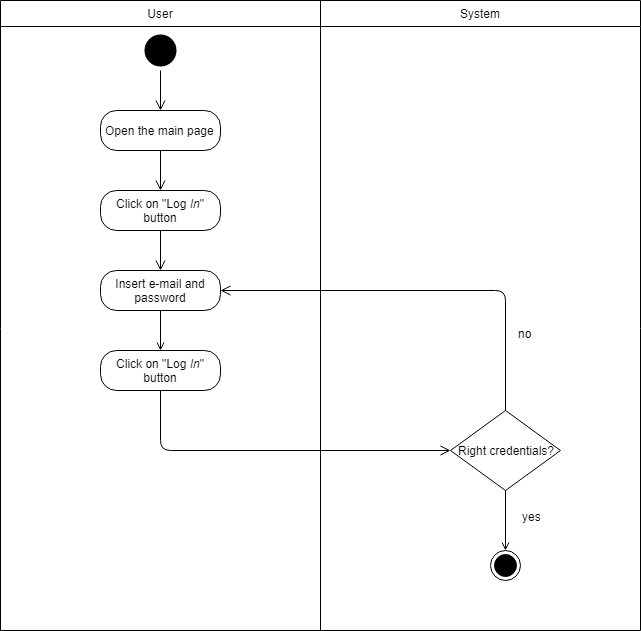
\includegraphics[width=\textwidth]{img/activity/IndividualLogin.png}
  \hspace{0.05\linewidth}
  \centering
  \caption{\textit{Generic Log In} activity diagram}
  \label{img:genericIndividualLoginActivityDiagram}
\end{center}
\end{figure}

\begin{figure}
\begin{center}
  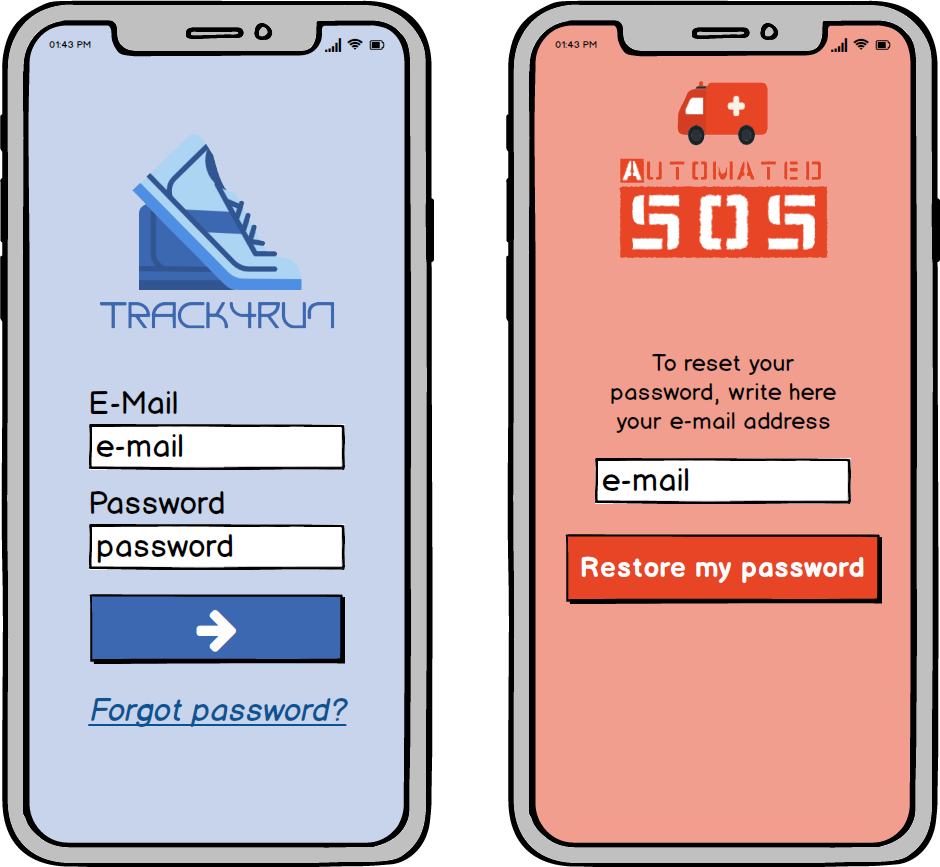
\includegraphics[width=\textwidth]{img/mockup/Generic_Login.png}
  \hspace{0.05\linewidth}
  \centering
  \caption{\textit{Generic Log In} mockup}
  \label{img:genericLogInMockup}
\end{center}
\end{figure}

\begin{center}
\begin{table}
\begin{tabular}{ | l | p{0.75\linewidth} | }
  \hline
    Actor & \textbf{Individual user} \\ \hline
    Goal & \textbf{[G.2]} \\ \hline
    Input Condition & The \textbf{Individual user} is already registered to the system and wants to log in \\ \hline
    Event Flow & \begin{minipage}[t]{0.7\textwidth}
      The first part of the event flow is already explained in Table \ref{table:genericIndividualLogInInTable}.
      \smallskip
      \begin{enumerate}
        \item The system asks the \textbf{Individual user} to turn on the bluetooth of the smartwatch and of the smartphone;
        \item The \textbf{Individual user} turns on the bluethooth;
        \item The system shows on the smartphone display the associable devices that it finds with the bluetooth connection;
        \item The \textbf{Individual user} selects the device he wants to associate.
        \item The \textbf{Individual user} clicks on "\textit{Done}" button.
      \end{enumerate}
    \smallskip
  \end{minipage} \\ \hline
  Output Condition & The system allows the \textbf{Individual user} to log in and loads his/her dashboard. \\ \hline
  Exceptions & \begin{minipage}[t]{0.7\textwidth}
    All already explained exceptions in Table \ref{table:genericIndividualLogInInTable} are still valid.
    \begin{itemize}
      \smallskip
      \item If the \textbf{Individual user} decides to leave the connecting device process this one is aborted.
    \end{itemize}
    \smallskip
  \end{minipage}  \\ \hline
\end{tabular}
\caption{\textit{First Individual Log In} use case}
\label{table:firstIndividualLogInInTable}
\end{table}
\end{center}

\begin{figure}
\begin{center}
  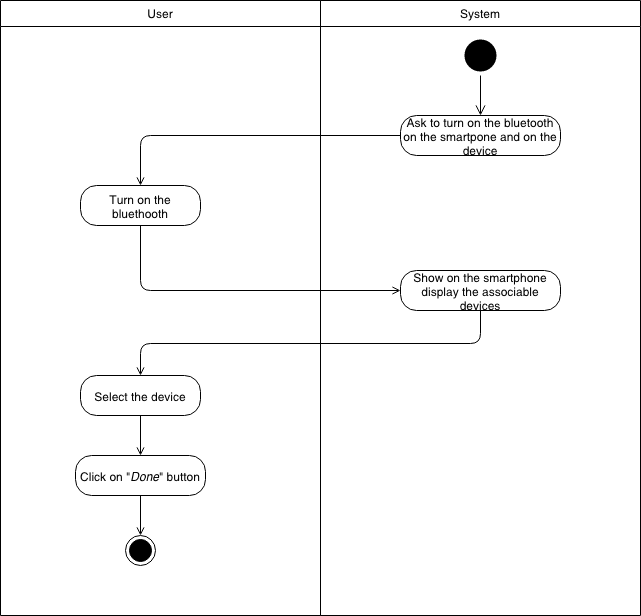
\includegraphics[width=\textwidth]{img/activity/FirstIndividualLogin.png}
  \hspace{0.05\linewidth}
  \centering
  \caption{\textit{First Log In} activity diagram}
  \label{img:firstIndividualLoginActivityDiagram}
\end{center}
\end{figure}

\begin{figure}
\begin{center}
  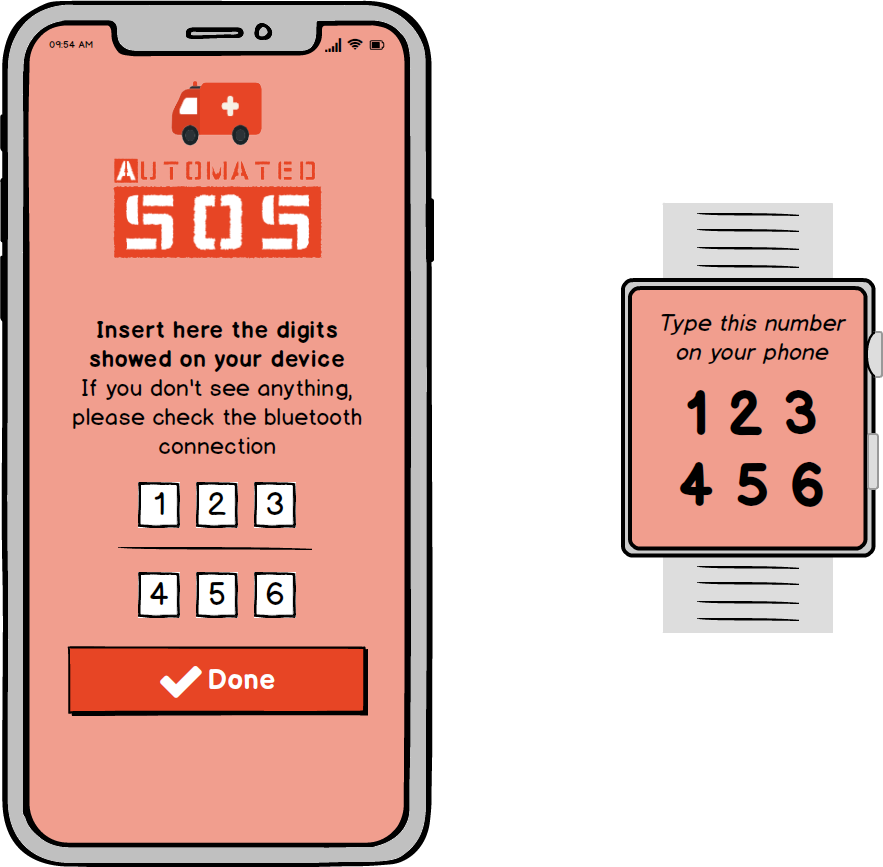
\includegraphics[width=\textwidth]{img/mockup/First_Login.png}
  \hspace{0.05\linewidth}
  \centering
  \caption{\textit{First Log In} mockup}
  \label{img:firstLogInMockup}
\end{center}
\end{figure}
